\documentclass[12pt]{standalone}
\usepackage{tikz}
%\usetikzlibrary{calc, arrows.meta, decorations.pathreplacing}

\begin{document}

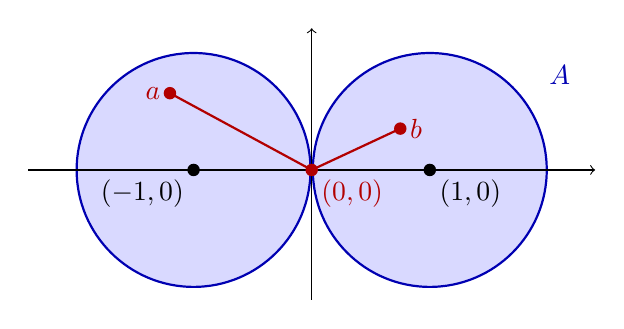
\begin{tikzpicture}[scale=1.5]
  \fill[blue!15] (-1,0) circle (0.98);
  \fill[blue!15] (1,0) circle (0.98);
  \draw[blue!70!black, thick] (-1,0) circle (0.99);
  \draw[blue!70!black, thick] (1,0) circle (0.99);

  \draw[->] (-2.4,0) -- (2.4,0); % node[right] {$x$};
  \draw[->] (0,-1.1) -- (0,1.2); % node[above] {$y$};

  \fill (-1,0) circle (1.5pt) node[below left] {$(-1,0)$};
  \fill (1,0) circle (1.5pt) node[below right] {$(1,0)$};
  \fill[red!70!black] (0,0) circle (1.5pt) node[below right] {$(0,0)$};
  % \fill (0,0) circle (1.5pt) node[above right] {$0$};

  \node[blue!70!black] at (2.1, 0.8) {$A$};

  \coordinate (a) at (-1.2, 0.65);
  \fill[red!70!black] (a) circle (1.5pt) node[left] {$a$};

  \coordinate (b) at (0.75, 0.35);
  \fill[red!70!black] (b) circle (1.5pt) node[right] {$b$};

  \draw[red!70!black, thick] (a) -- (0,0) -- (b);
\end{tikzpicture}

\end{document}
